\documentclass[t,compress]{beamer}
\usepackage[cp1250]{inputenc}
\usepackage[T1]{fontenc}
\usepackage[polish]{babel}
\usepackage{color}
\usepackage{xmpmulti}
\usepackage{multimedia}
\setbeamertemplate{bibliography item}[text] %default is an icon of an article 

\setbeamercolor{section in head/foot}{use=structure,bg=structure.fg!25!bg}

\useoutertheme[subsection=true]{miniframes}

\setbeamertemplate{frametitle}[default][center]

\AtBeginDocument{%
  {    \usebeamercolor{section in head/foot}
  }
  
  \pgfdeclareverticalshading{beamer@headfade}{\paperwidth}
  {%
    color(0cm)=(bg);
    color(1.25cm)=(section in head/foot.bg)%
  }

  \setbeamercolor{section in head/foot}{bg=}
}

\addtoheadtemplate{\pgfuseshading{beamer@headfade}\vskip-1.25cm}{}

\beamertemplatedotitem


\title[Poznan University of Technology]{Poznan University of Technology}
\author[Institute of Control and Information Engineering]{%
  Institute of Control and Information Engineering\inst{ }
}
\institute[Reasearch activities]{
   \inst{ }%
  Reasearch activity
}
\date[07.11.2012]{Pozna\'n, 07.11.2012}
\subject{temat}

\pgfdeclaremask{tu}{images/Logo-PP-mask}
\pgfdeclaremask{ur}{images/logo-iaii-mask}
\pgfdeclareimage[mask=tu,width=0.6cm]{Logo-PP}{images/Logo-PP}
\pgfdeclareimage[mask=ur,width=1cm]{logo-iaii}{images/logo-iaii}

\logo{\vbox{\hbox to 1cm{\hfil\pgfuseimage{Logo-PP}}\vskip0.1cm\hbox{\pgfuseimage{logo-iaii}}}}


\begin{document}

\frame{\titlepage}

\part<presentation>{Main Talk}

%\begin{frame}
%  \frametitle{Control of walking robots}

%  \begin{columns}

%    \column{4.7cm}
%      \begin{figure}[h]
%	  \centering      \includegraphics[width=1.0\columnwidth]{images/messor}      
%      \end{figure}
	
%  \column{5.8cm}
%        \begin{block}{Mobile Robotics Lab research topics}
%	  \begin{itemize}
%	   \item Stairs negotiation~\cite{iros2012kw}
%	   \item Integrated motion planning~\cite{iros2012}
%	   \item Learning foothold selection~\cite{jfr2011, icra2010}
%	   \item Static stability analysis~\cite{amcs2011}
%	   \item Learning the gait cycle~\cite{amcs2010}%, iros2008}
%	  \end{itemize}

%        \end{block}
%  \end{columns}
%\end{frame}

% \begin{frame}
%   \frametitle<presentation>{Results}
%    \begin{center}
%     \movie[width=8cm,height=5.8cm,externalviewer]{\includegraphics[width=0.75\textwidth]{images/messor2}}{movies/Messor_CIE.avi}                                                                                                                               \end{center}
% \end{frame}

%\begin{frame}
%  \frametitle{Control of walking robots -- results}

%  \begin{columns}

%    \column{4.7cm}
%   \begin{center}
%    \movie[width=4.6cm,height=3.8cm,externalviewer]{\includegraphics[width=1.0\columnwidth]{images/messor2}}{movies/Messor_CIE.avi}                                                                                                                               \end{center}
	
%  \column{5.8cm}
%        \begin{block}{Messor robot}
%	  \begin{itemize}
%	   \item No. of legs: 6
%	   \item Length: 30.6 cm
%	   \item Width: 26.0 cm
%	   \item Weight: 4.3~kg
%	   \item Sensors: Laser scanner URG-04LX, AHRS XSense MTi, Video camera UI-1225
%	  \end{itemize}

%        \end{block}
%  \end{columns}
%\end{frame}

%\begin{frame}
%  \frametitle{References}
  
%\begin{scriptsize}
%\bibliographystyle{unsrt}

%\begin{thebibliography}{99}
%\bibitem[1]{iros2012kw} K. Walas, Discrete Event Controller for Urban Obstacles Negotiation with Walking Robot, IEEE/RSJ 2012 International Conference on Intelligent Robots and Systems, Vilamoura, Portugal, 2012
%\bibitem[2]{iros2012} D. Belter, P. Skrzypczy\'nski, Posture Optimization Strategy for a Statically Stable Robot Traversing Rough Terrain, IEEE/RSJ 2012 International Conference on Intelligent Robots and Systems, Vilamoura, Portugal, 2012
%\bibitem[3]{jfr2011} D. Belter, P. Skrzypczy\'nski, Rough terrain mapping and classification for foothold selection in a walking robot, Journal of Field Robotics, vol. 28(4), pp. 497--528, 2011
%\bibitem[4]{icra2010} D. Belter, P. Labecki, P. Skrzypczy\'nski, Map-based Adaptive Foothold Planning for Unstructured Terrain Walking, 2010 IEEE International Conference on Robotics and Automation, Anchorage, Alaska, USA, pp.~5256--5261, 2010
%\bibitem[5]{amcs2011} K. Walas, D. Belter, Supporting locomotive functions of a six-legged walking robot, International Journal of Applied Mathematics and Computer Science, vol.~21(2), pp.~363--377, 2011
%\bibitem[6]{amcs2010}D. Belter, P. Skrzypczy\'nski, A Biologically Inspired Approach to Feasible Gait Learning for a Hexapod Robot, International Journal of Applied Mathematics and Computer Science, Vol.~20(1), pp.~69--84, 2010
% \bibitem[7]{iros2008}D. Belter, A. Kasi\'nski, P. Skrzypczy\'nski, Evolving Feasible Gaits for a Hexapod Robot by Reducing the Space of Possible Solutions, IEEE/RSJ 2008 International Conference on Intelligent Robots and Systems, Nice, France, pp.~2673--2678, 2008 
%\end{thebibliography}
%\end{scriptsize}

%\end{frame}

\begin{frame}
	\frametitle{The Isfar Project}
	\begin{center} A hybrid of ROV/AUV classes vehicle designed for the inland underwater exploration
    \movie[width=8cm,height=5.8cm,externalviewer]{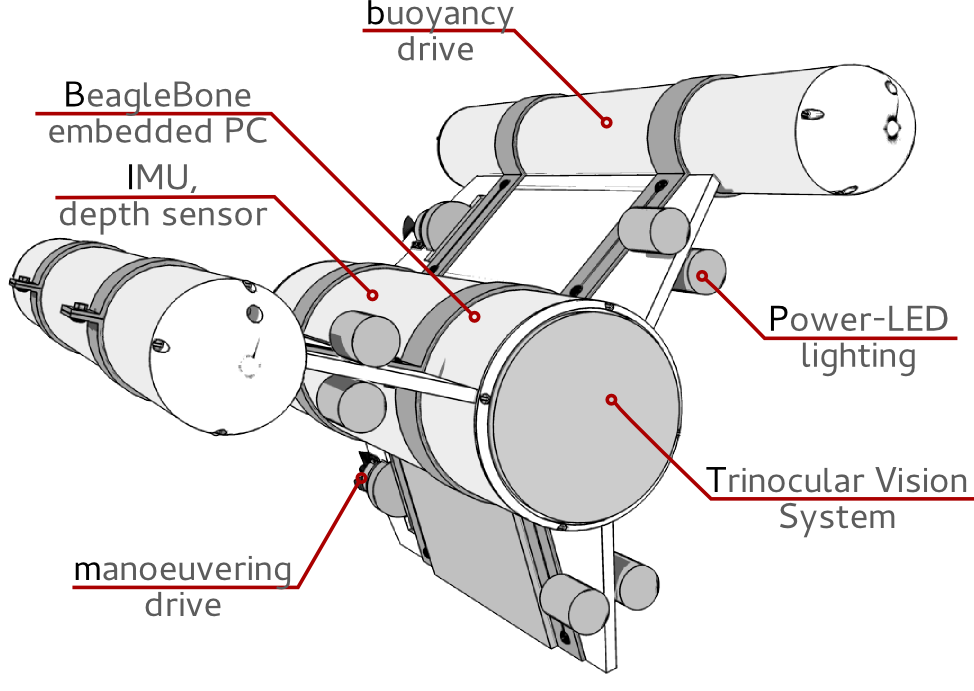
\includegraphics[width=0.75\textwidth]{images/robotisfar}}{movies/isfar.mp4} \end{center}
\end{frame}

\begin{frame}
	\frametitle{The Isfar Project}
	Parameters:\\
	\begin{itemize}
		\item operating depth: 20 m,
		\item linear velocity: 5 km/s,
		\item weight: 20 kg,
		\item dimensions: (0.6 x 0.9 x 0.4) m
	\end{itemize}
	Applications:\\
	\begin{itemize}
		\item underwater searching missions - lake/river bed scanning and mapping,
		\item environmental observation, water quality survey, searching for the sources of the water contamination,
		\item support in rescue missions,
		\item inspection of underwater constructions,
		\item archeological search
	\end{itemize}
	\movie[]{}{}
\end{frame}
	
\begin{frame}
	\frametitle{The Isfar Project}
	Scientific problems:\\
	\begin{itemize}
		\item Control of a 6 DoF underwater vehicle in the terms of disturbances such as river currents.
		\item Multimodal (NIR, VIS and NUV bands) image registration and data fusion algorithms for underwater imaging purposes.
	\end{itemize}
	References:\\
	\begin{scriptsize}
	\bibliographystyle{unsrt}
	\begin{thebibliography}{99}
		\bibitem[1]{jamris} W. Biega\'nski, J. Ceranka, A. Kasi\'nski , Design, control and applications of the underwater robot Isfar, Journal of Automation, Mobile Robotics \& Intelligent Systems, 02/2011, pp. 60 - 65
		\bibitem[2]{zeszyty} J. Ceranka, Motion Simulation and Visualisation of the Underwater Object, Poznan University of Technology Academic Journals of Electrical Engineering, 66, pp. 163 - 168, 2011
	\end{thebibliography}
\end{scriptsize}
\end{frame}


\end{document}
